\section{Résultats obtenus}
	L'application finale permet de personnaliser différentes choses. Une interface graphique permet d'effectuer ces personnalisations avant de lancer la simulation (Figure~\ref{fig:personnalisation}). Les personnalisations possibles sont les suivantes :
	
	\begin{enumerate}
		\item La position de la (ou des) sorties
		\item Le placement des obstacles au sein de la pièce
		\item La position des personnes présentes dans la pièce
	\end{enumerate}		

	\begin{figure}[H]
	\centering
	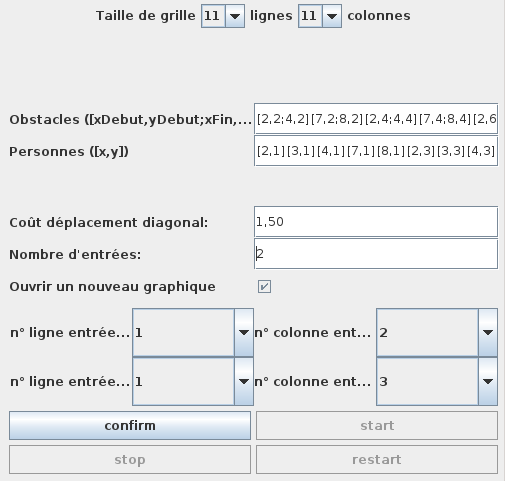
\includegraphics[scale=0.7]{imagesPNG/personnalisation.png}
	\caption{Représentation des distances parcourues\label{fig:personnalisation}}
	\end{figure}
		
	Une fois cette personnalisation effectuée et validée, la grille est générée, et les fenêtres contenant les diagrammes s'ouvrent en parallèle. L'utilisateur n'a plus qu'à cliquer sur le bouton "Start" pour démarrer la simulation de l'évacuation. Cette dernière continuera jusqu'à ce que l'évacuation soit complète, en mettant à jour les diagrammes en temps réel. A la fin de la simulation, le programme ajoute la date de sortie de la dernière personne de façon à pouvoir comparer les temps d'évacuation de différentes configurations ou la variation de cette date pour une même configuration selon le comportement aléatoire des personnes. On notera également que l'utilisateur a la possibilité de stopper la simulation grâce au bouton "Stop". \\
	
	La Figure~\ref{fig:captureGlobale} montre l'affichage lorsqu'une simulation est en cours. La Figure~\ref{fig:dateSortie} montre une courbe représentant les dates de sortie des dernières personnes de plusieurs simulations. Pour le relevé de ces valeurs, les positions des sorties ont toujours été les m\^emes. Ces configurations sont schématisées sur la Figure~\ref{fig:configMesures}. A chaque fois, on ajoutais une ouverture : pour une seule sortie, seule la case 1 était libre; pour deux sorties, les cases 1 et 2 étaient libres, etc...

	\begin{figure}[H]
	\centering
	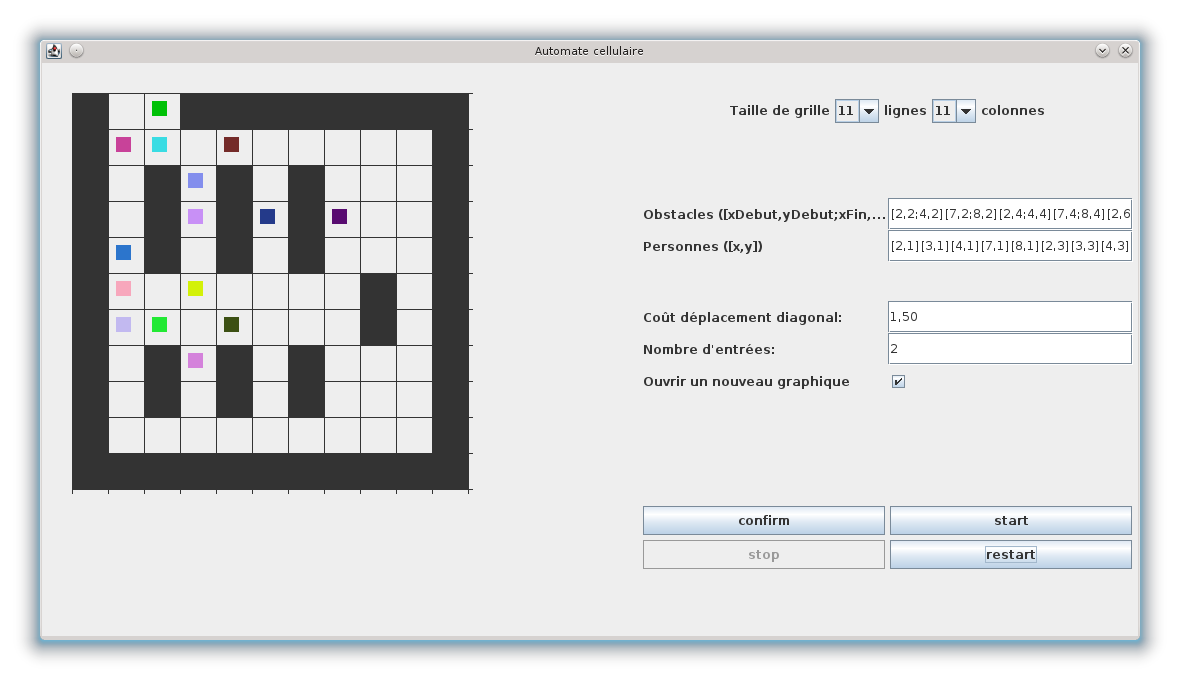
\includegraphics[scale=0.4]{imagesPNG/captureGlobale.png}
	\caption{Représentation des distances parcourues\label{fig:distances_parcourues}}
	\end{figure}
	
	\begin{figure}[H]
	\centering
		\begin{tikzpicture}[y=.2cm, x=.7cm,font=\sffamily]
		 	%axis
			\draw (0,0) -- coordinate (x axis mid) (10,0);
		    	\draw (0,0) -- coordinate (y axis mid) (0,30);
		    	%ticks
		    	\foreach \x in {0,...,10}
		     		\draw (\x,1pt) -- (\x,-3pt)
					node[anchor=north] {\x};
		    	\foreach \y in {0,5,...,30}
		     		\draw (1pt,\y) -- (-3pt,\y) 
		     			node[anchor=east] {\y}; 
			%labels      
			\node[below=0.8cm] at (x axis mid) {Nb de sorties};
			\node[rotate=90, above=0.8cm] at (y axis mid) {Durées d'évacuation};
		
			%plots
			\draw plot[mark=*, mark options={fill=white}] 
				file {duree_evac.data};
			\draw plot[mark=square*, mark options={fill=red}] 
				file {duree_evac2.data};
				
			%legend
			\begin{scope}[shift={(4,4)}]
		%	\draw (0,0) -- 
		%		plot[mark=*, mark options={fill=white}] (0.25,0) -- (0.5,0) 
		%		node[right]{Série 1};
		%	\draw[yshift=\baselineskip] (0,0) -- 
		%		plot[mark=square*, mark options={fill=red}] (0.25,0) -- (0.5,0)
		%		node[right]{Série 2};
			\end{scope}
		\end{tikzpicture}	
	\caption{Durées d'évacuation en fonction du nombre de sorties \label{fig:dateSortie}}
	\end{figure}

	\begin{figure}[H]
	\centering
	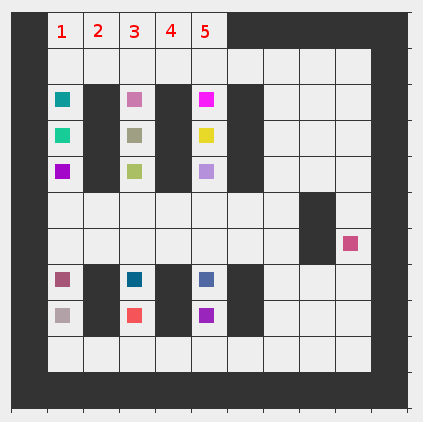
\includegraphics[scale=0.4]{imagesPNG/grille2.png}
	\caption{Configuration utilisée pour les mesures\label{fig:configMesures}}
	\end{figure}